\documentclass[journal]{IEEEtran}

\usepackage[numbers,sort&compress]{natbib}
\usepackage{amsmath,amssymb,amsfonts,amsthm}
\usepackage{mathtools}
\usepackage{graphicx}
\usepackage{booktabs}
\usepackage{xcolor}
\usepackage{pgfplots}
\pgfplotsset{compat=1.17}
\usepackage{xurl}
\usepackage{xr-hyper}
\usepackage[hidelinks]{hyperref}
\externaldocument[M-]{main}

\newtheorem{theorem}{Theorem}
\newtheorem{proposition}[theorem]{Proposition}
\newtheorem{corollary}[theorem]{Corollary}
\newtheorem{lemma}[theorem]{Lemma}
\theoremstyle{definition}
\newtheorem{definition}{Definition}
\newtheorem{assumption}{Assumption}
\theoremstyle{remark}
\newtheorem{remark}{Remark}

\newcommand{\F}{\mathcal{F}}
\newcommand{\KL}{\mathrm{KL}}
\newcommand{\Bern}{\mathrm{Bern}}
\newcommand{\eps}{\varepsilon}
\newcommand{\TV}{\mathrm{TV}}

\begin{document}

\title{Supplementary Material for\\ ``Canary-Aware Providers and the Limits of Unlearning
Audits: A Sharp Bound and the Detectability--Power Trade-off''}
\author{Quang-Vinh~Dang}
\maketitle

% Numbering continues from the main manuscript.
\setcounter{table}{6}
\setcounter{figure}{0}
\setcounter{theorem}{7}
\renewcommand{\thesection}{S-\Roman{section}}
\renewcommand{\theequation}{S\arabic{equation}}

This supplement contains the proofs omitted from the main text
(Section~\ref{sec:s-proofs}), a bound on the certification time of the cohort certificate
that the main text refers to (Section~\ref{sec:s-time}), and additional experimental results
(Section~\ref{sec:s-results}). Numbering of theorems, tables and figures continues that of the
main manuscript.

\section{Proofs}\label{sec:s-proofs}

\subsection{Proof of Theorem~\ref{M-thm:population}}

Given $\xi$, $\Delta$ is a function of the $2m$ independent coordinates
$(b_1,\dots,b_m,C_1,\dots,C_m)$. By Assumption~\ref{M-ass:influence}, changing one coin changes
$\Delta$ by at most $2\kappa/m$ and changing one pair's contents by at most $2\ell/m$.
McDiarmid's inequality \citep{mcdiarmid1989bounded} gives
$\Pr[|\Delta-\Delta_\xi|\ge u]\le2\exp(-2u^2/\sum_kc_k^2)$ with
$\sum_kc_k^2=4(\kappa^2+\ell^2)/m$, that is $2\exp(-u^2m/(2(\kappa^2+\ell^2)))$; equating it to
$\alpha'$ gives $u_m$. Corollary~\ref{M-cor:ladder} follows by a union bound with the
certificate's error probability and Theorems~\ref{M-thm:detect} and~\ref{M-thm:sharp}. Under exact
unlearning $\kappa=\ell=1$, since a pair's coin or contents can then affect only that pair's
own term. Under partial unlearning $\kappa$ and $\ell$ measure how far one canary's training
reaches into the others' scores; with stochastic training one record can perturb every pair
whose score difference is close to zero, so the assumption is a worst-case bound that the
auditor cannot check.

\subsection{Proof of Proposition~\ref{M-prop:semantic}}

Write $\F_{t-1}$ for the auditor's information after $t-1$ reveals.
\begin{proof}
We follow the proof of \cite[Thm.~1]{dang2026vouch}. Enlarge $\F_{t-1}$ to $\mathcal G_{t-1}$,
which also reveals the position $\pi(t)$ and the \emph{unordered} contents
$\{c^0_j,c^1_j\}$ of the pair $j=\pi(t)$ opened at step $t$, but not its coin. Given
$\mathcal G_{t-1}$ and the deployed model, the two numbers $s(M,c^0_j)$ and
$s(M,c^1_j)$ are determined, because each score is a function of the model and the
record alone: both twins share the literal prefix or the question set $Q$ and differ only
in the value evaluated, and the calibrated score subtracts $s(M_0,\cdot)$, where the base
model $M_0$ is fixed before any coin is drawn. The coin $b_j$ is independent of the other
coins and of the contents by Assumption~\ref{M-ass:gen}, independent of $M$ given the
contents by hypothesis, and no earlier reveal involves it, so
$b_j\mid\mathcal G_{t-1}\sim\Bern(\frac12)$. Since $b_j$ decides which of the two
determined numbers is the in-twin's, $D_j\overset{d}{=}-D_j$ given $\mathcal G_{t-1}$,
and the committed tie-break coin splits an atom at zero equally, so
$Z_j\mid\mathcal G_{t-1}\sim\Bern(\frac12)$. Averaging over
$\mathcal G_{t-1}\supseteq\F_{t-1}$ gives the claim. The semantics of the records never
enters.
\end{proof}

\subsection{Proof of Proposition~\ref{M-prop:class}}

Write $E_s$ for the wealth process of arm $s$ and $E=\sum_sw_sE_s$.
\begin{proof}
(i) The proof of \cite[Thm.~2]{dang2026vouch} conditions on the sign vectors of all scores and, given a
violated tolerance of some score $s^\ast$, bounds the probability that $E_{s^\ast}$ ever
reaches $1/\alpha$ by $\alpha$; the false certificate requires that event, so no union
over $\F'$ is needed. Issuance needs every arm to cross, hence the maximum of the crossing
times. (ii) A weighted average of supermartingales is a supermartingale
\citep[the merging of e-values by averaging;][]{vovk2021evalues}. If
$E_s\ge1/(w_s\alpha)$ then $E\ge w_sE_s\ge1/\alpha$. (iii) Apply
Proposition~\ref{M-prop:anytime}(ii) to $w E_{s^\ast}$ crossing $1/\alpha$, that is
$E_{s^\ast}$ crossing $1/(w\alpha)$.
\end{proof}

\subsection{The price of continuous monitoring}

A provider under audit may be monitored at any time, so the auditor needs a test that stays
valid under optional stopping. In the sign model, i.i.d.\ signs $Z_t\sim
\Bern(\frac{1+\Delta}2)$ tested against $\Delta=0$, let
$\KL(\Delta)=\frac{1+\Delta}2\log(1+\Delta)+\frac{1-\Delta}2\log(1-\Delta)\approx\Delta^2/2$.

\begin{proposition}[Expected stopping time]\label{prop:anytime}
(i) Every level-$\alpha$ sequential test that stops almost surely under $\Delta$ has
$\mathbb{E}_\Delta\tau\ge\log(1/\alpha)/\KL(\Delta)$. (ii) The oracle bettor with stake
$\Delta$ stops with $\mathbb{E}_\Delta\tau\le(\log(1/\alpha)+\log(1+\Delta))/\KL(\Delta)$.
(iii) A uniform mixture of $K$ constant stakes $\lambda_k$ stops with
$\mathbb{E}_\Delta\tau\le(\log(K/\alpha)+\log(1+\lambda_k))/g_\Delta(\lambda_k)$ for every $k$
with $g_\Delta(\lambda_k)=\frac{1+\Delta}2\log(1+\lambda_k)+\frac{1-\Delta}2\log(1-\lambda_k)
>0$.
\end{proposition}


\begin{proof}[Proof of Proposition~\ref{prop:anytime}]


(i) Let $\Lambda_t=\sum_{u\le t}\log\frac{d\Bern((1+\Delta)/2)}{d\Bern(1/2)}(Z_u)$. Wald's
identity \citep{wald1945sequential} gives $\mathbb{E}_\Delta\Lambda_\tau=\mathrm{KL}(\Delta)\,\mathbb{E}_\Delta\tau$.
Changing measure on $\{\tau=n\}$, where $d\Pr_0/d\Pr_\Delta=e^{-\Lambda_n}$,
$\alpha\ge\Pr_0[\tau<\infty]=\mathbb{E}_\Delta\bigl[e^{-\Lambda_\tau}\bigr]\ge
e^{-\mathbb{E}_\Delta\Lambda_\tau}$ by Jensen, so $\mathbb{E}_\Delta\Lambda_\tau\ge
\log(1/\alpha)$.
(ii) $W_t$ is a nonnegative martingale under the null with $W_0=1$, so Ville's inequality
gives level $\alpha$. Under $\Delta$, $\mathbb{E}\log(1+\Delta(2Z-1))=\frac{1+\Delta}2
\log(1+\Delta)+\frac{1-\Delta}2\log(1-\Delta)=\mathrm{KL}(\Delta)=:g$, and
$\log W_t-gt$ is a martingale with bounded increments, so Wald's identity gives
$\mathbb{E}\log W_\tau=g\,\mathbb{E}\tau$ once $\mathbb{E}\tau<\infty$, which holds since the
drift is positive. Since $W_{\tau-1}<1/\alpha$ and each factor is at most $1+\Delta$,
$\log W_\tau<\log(1/\alpha)+\log(1+\Delta)$.
(iii) The mixture wealth is at least $W^{\lambda_k}_t/K$, so it crosses $1/\alpha$ no later
than $W^{\lambda_k}$ crosses $K/\alpha$; apply (ii) with $\alpha\to\alpha/K$ and the stake
$\lambda_k$, whose growth rate is $g_\Delta(\lambda_k)$; the proof of (ii) applies verbatim
to any stake with positive growth rate, with overshoot factor $1+\lambda_k$.
\end{proof}


Table~\ref{tab:anytime} checks the constants by simulation. A two-sided sequential test runs
two arms at level $\alpha/2$, so its oracle expected time is $2\log(2/\alpha)/\Delta^2\,(1+o(1))$
as $\Delta\to0$, while the two-sided fixed-sample sign test needs
$n\approx(z_{1-\alpha/2}+z_{1-\beta})^2/\Delta^2$ pairs for power $1-\beta$. At $\alpha=0.05$
the constants are $7.4$ for the sequential oracle and $3.8$, $7.9$, $10.5$ for power $0.5$,
$0.8$, $0.9$.

\begin{table}[t]
\centering\small
\caption{Expected sample sizes in the sign model, $\alpha=0.05$ (one arm at level
$0.025$, as in each direction of a two-sided test). Arm Wald: lower bound of
Proposition~\ref{M-prop:anytime}(i) for the arm; oracle: bound (ii) and simulated mean over
$2{,}000$ runs, which may exceed the bound by Monte Carlo error (standard error about
$1.6\%$ of the mean); grid: simulated mean of the $10$-stake constant mixture over $500$
runs; $n_{50},n_{80},n_{90}$: smallest $n$ for which the exact two-sided binomial
sign test at level $0.05$ has the stated power.}
\label{tab:anytime}
\resizebox{\columnwidth}{!}{\begin{tabular}{rrrrrrrrr}
\toprule
$\Delta$ & KL & arm Wald & oracle $\le$ & oracle sim. & grid sim. & $n_{50}$ & $n_{80}$ & $n_{90}$ \\
\midrule
0.05 & 0.0013 & 2950 & 2989 & 2990 & 4225 & 1590 & 3234 & 4259 \\
0.10 & 0.0050 & 737 & 756 & 749 & 952 & 409 & 809 & 1112 \\
0.20 & 0.0201 & 183 & 192 & 186 & 211 & 103 & 204 & 284 \\
0.30 & 0.0457 & 81 & 86 & 81 & 98 & 47 & 95 & 123 \\
0.50 & 0.1308 & 28 & 31 & 30 & 34 & 17 & 33 & 43 \\
\bottomrule
\end{tabular}
}
\end{table}

\section{Certification time of the cohort certificate}\label{sec:s-time}

VOUCH bounds the certification time through refutation: once enough zeros have been revealed
the null becomes infeasible \citep{dang2026vouch}. In practice the wealth crosses $1/\alpha$
much earlier, by growth. Under a uniform reveal order $\pi$ the upper arm bets against the
without-replacement boundary
\begin{equation}\label{eq:worboundary}
p_0(t)=\frac{mp_0-S_{t-1}}{m-t+1},\qquad p_0=\tfrac12+\tfrac\eps2,
\end{equation}
with wealth $W_t=\prod_{u\le t}(1+\lambda_u(p_0(u)-Z_{\pi(u)}))$, and $\F_t$ denotes the
auditor's information after $t$ reveals.

\begin{lemma}[Deterministic edge]\label{lem:edge}
Consider the upper certificate arm with $p_0=\frac12+\frac\eps2$. Let the cohort carry
$j$ ones, $\hat p=j/m<p_0$, and $\delta=p_0-\hat p$. Under a uniform reveal order, the
boundary $p_0(t)$ of~\eqref{eq:worboundary} and the conditional mean
$r_t=\mathbb{E}[Z_{\pi(t)}\mid\F_{t-1}]$ satisfy, for every $t$ and every history,
\[
g_t \;:=\; p_0(t)-r_t \;=\; \frac{m\delta}{m-t+1}.
\]
\end{lemma}

\begin{proof}
With $S_{t-1}$ ones revealed, $p_0(t)=(mp_0-S_{t-1})/(m-t+1)$ and, since the unrevealed
remainder is a uniformly ordered set containing $j-S_{t-1}$ ones,
$r_t=(j-S_{t-1})/(m-t+1)$. Subtracting cancels $S_{t-1}$.
\end{proof}

The edge grows as the cohort is exhausted. On an i.i.d.\ stream with the same mean it
would stay equal to $\delta$; the growth is the finite-population advantage of the
cohort target.

\begin{theorem}[Certification time through wealth growth]\label{thm:growth}
Fix the realised cohort, with $j$ ones and $\delta=p_0-\hat p>0$ as in
Lemma~\ref{lem:edge}, so that the only randomness is the uniform reveal order. Run the
upper arm with a uniform mixture of $K$ constant stakes
$\Lambda=\{\lambda_1,\dots,\lambda_K\}\subset(0,\frac12]$, refuting the null outright if
$p_0(t)>1$. Let $H_n$ denote the harmonic numbers,
\begin{align*}
A_t&=\sum_{u\le t}g_u=m\delta\,(H_m-H_{m-t}),\\
G_t&=\sum_{u\le t}g_u^2=m^2\delta^2\!\!\sum_{k=m-t+1}^{m}\!k^{-2},
\end{align*}
and for $\lambda\in\Lambda$
\begin{align*}
\Psi_t(\lambda)&=\lambda A_t-\frac{\lambda^2(t/4+G_t)}{2(1-\lambda)^2},\\
V_t(\lambda)&=\frac{\lambda^2(t/4+G_t)}{(1-\lambda)^2},\qquad
R_\lambda=\log\frac{1+\lambda}{1-\lambda}.
\end{align*}
Then the stopping time $\tau$ of the arm (wealth reaching $1/\alpha$, or refutation)
satisfies, for every $t<m$,
\[
\Pr[\tau>t]\;\le\;\min_{\lambda\in\Lambda}
\exp\!\Bigl(-\frac{x_t(\lambda)^2}{2\bigl(V_t(\lambda)+R_\lambda x_t(\lambda)/3\bigr)}\Bigr),
\]
where $x_t(\lambda)=\bigl(\Psi_t(\lambda)-\log(K/\alpha)\bigr)_+$.
\end{theorem}

\begin{proof}
Fix $\lambda\in\Lambda$ and let $X_u=\log\bigl(1+\lambda(p_0(u)-Z_{\pi(u)})\bigr)$,
so that $\log W^\lambda_t=\sum_{u\le t}X_u$. Before refutation $p_0(u)\in[0,1]$, so
$y_u=\lambda(p_0(u)-Z_{\pi(u)})\in[-\lambda,\lambda]$. By Taylor's theorem with
remainder, $\log(1+y)\ge y-y^2/(2(1-\lambda)^2)$ for $y\ge-\lambda$. Hence
$\mathbb{E}[X_u\mid\F_{u-1}]\ge\lambda g_u-\lambda^2\,\mathbb{E}[(p_0(u)-Z_{\pi(u)})^2\mid
\F_{u-1}]/(2(1-\lambda)^2)$, and
$\mathbb{E}[(p_0(u)-Z_{\pi(u)})^2\mid\F_{u-1}]=r_u(1-r_u)+g_u^2\le\frac14+g_u^2$.
Summing over $u\le t$, the compensator of $\log W^\lambda_t$ is at least
$\Psi_t(\lambda)$, a deterministic quantity by Lemma~\ref{lem:edge}. Further,
$|\log(1+y)|\le|y|/(1-\lambda)$ for $|y|\le\lambda$, so the conditional variances of
the $X_u$ sum to at most $V_t(\lambda)$, and the centred increments are bounded below by
$-R_\lambda$. After refutation, replace $X_u$ by its compensator lower bound, so that the
centred sequence remains a martingale difference sequence; this changes nothing on the
event that refutation has not occurred by $t$. Freedman's inequality
\citep{freedman1975tail}, applied to the negated increments, gives
$\Pr[\log W^\lambda_t<\Psi_t(\lambda)-x]\le\exp\bigl(-x^2/(2(V_t(\lambda)+R_\lambda
x/3))\bigr)$. Finally, the mixture wealth is at least $W^\lambda_t/K$, so on the event of
no refutation by $t$ we have $\{\tau>t\}\subseteq\{\log W^\lambda_t<\log(K/\alpha)\}$.
Taking $x=x_t(\lambda)$ and minimising over $\Lambda$ completes the proof.
\end{proof}

\paragraph{Reading the bound.} Since $1/(m-u+1)\ge1/m$, $A_t\ge\delta t$, with equality
only in the limit of an infinite cohort; the factor $\rho_t=m(H_m-H_{m-t})/t\approx
1+t/(2m)$ is the finite-population speed-up. Ignoring $G_t$ and the factor
$(1-\lambda)^{-2}$ and optimising $\lambda$, the drift is about $2\delta^2t\rho_t^2$, so
the time scale is $t^\ast\approx\log(K/\alpha)/(2\delta^2\rho_{t^\ast}^2)$, against
$\log(1/\alpha)/\KL\approx\log(1/\alpha)/(2\delta^2)$ for an i.i.d.\ stream. The original
study found its cohort certificate faster than the super-population one at every
tolerance and attributed this to the cap at cohort exhaustion, where the claim resolves
deterministically. The bound shows that the speed-up starts well before exhaustion,
through the edge that grows as the cohort runs out. The lower arm is the mirror
statement with $\delta'=\hat p-(1-p_0)$, and the two-sided certificate needs both arms.
The theorem covers a constant-stake mixture. VOUCH's engine uses adaptive experts
(online Newton step, Krichevsky--Trofimov); if the engine's wealth were a uniform
average over its experts with the constant-stake grid among them, the same argument
would apply with $K$ replaced by the total number of experts, but we do not prove a
bound for the adaptive experts themselves, and the numerical check below runs the
constant-stake mixture, not the engine.

\paragraph{Scope.} The bound conditions on the realised cohort and is therefore not a
sample-size rule fixed in advance: $\delta$ depends on the cohort's own advantage. It
covers one arm of one score. A two-sided certificate over a class $\F$ is issued when
all $2|\F|$ arms have crossed, so its time is the maximum of the arm times and, by a
union bound, $\Pr[\tau_{\mathrm{cert}}>t]$ is at most the sum of the $2|\F|$ arm
bounds.

\paragraph{Numerical check.} We compare the bound with the empirical tail of the same
mixture bettor ($K=10$ stakes, $0.05,0.10,\dots,0.50$) over $2{,}000$ uniformly random orders, at $\hat p=\frac12$
and $(m,\eps)\in\{(512,0.2),(1024,0.2),(1024,0.1),(2048,0.1)\}$
(Table~\ref{tab:growth}). The bound is never violated at any of the $32$ checked times
per setting. It is conservative: the first time at which it falls below one half is
$2.2$ to $3.8$ times the empirical median. The same bettor against a fixed boundary on
an i.i.d.\ stream with the same mean is slower in every setting.


\begin{table}[t]
\centering\small
\caption{Certification time of the upper arm, $\hat p=\frac12$, $\alpha=0.05$,
$2{,}000$ uniformly random reveal orders per setting. ``Bound $\le\frac12$'' is the first
checked time at which Theorem~\ref{thm:growth} bounds $\Pr[\tau>t]$ by one half;
``fixed boundary'' is the same bettor on an i.i.d.\ stream with the same mean.}
\label{tab:growth}
\resizebox{\columnwidth}{!}{\begin{tabular}{rrrrrrr}
\toprule
$m$ & $\eps$ & median $\tau$ & bound $\le\frac12$ & ratio & fixed boundary & violations \\
\midrule
512 & 0.2 & 119 & 346 & 2.9 & 142 & 0/32 \\
1024 & 0.2 & 130 & 490 & 3.8 & 138 & 0/32 \\
1024 & 0.1 & 370 & 810 & 2.2 & 527 & 0/32 \\
2048 & 0.1 & 427 & 1226 & 2.9 & 532 & 0/32 \\
\bottomrule
\end{tabular}
}
\end{table}


\section{Additional experimental results}\label{sec:s-results}

\subsection{Auditing with semantic twins}\label{sec:exp-semantic}


Before turning to matched canaries we check that semantic twins give a working audit when
canaries are repeated as in VOUCH and the forget set contains every trained form
(Table~\ref{tab:semantic}). Paraphrased questions that were never trained carry most of the
literal advantage ($0.24$ against $0.28$ on average, calibrated), and the audit over all
scores revokes the positive control and issues for retraining in every seed at $\eps=0.2$;
GA and NPO remove both advantages. A GPT-2 pilot did not separate the controls: semantic
twins need a model that generalises a stated fact to its paraphrases.

\begin{table}[t]
\centering\footnotesize\setlength{\tabcolsep}{2.5pt}
\caption{Semantic-twin audit on Pythia-410M, full forget set, $m=384$, three seeds: realised
calibrated literal and paraphrase advantages per seed and the two-sided verdict (I issued, R
revoked, U undetermined).}
\label{tab:semantic}
\resizebox{\columnwidth}{!}{\begin{tabular}{lllcc}
\toprule
Subject & literal $\hat\Delta$ & paraphrase $\hat\Delta$ & $\eps=0.2$ & $\eps=0.1$ \\
\midrule
no unlearning & $+0.22$, $+0.31$, $+0.30$ & $+0.20$, $+0.27$, $+0.26$ & R R R & R R R \\
GA (100 steps) & $+0.04$, $+0.05$, $-0.09$ & $+0.05$, $+0.05$, $-0.07$ & I I I & I I I \\
NPO (250 steps) & $+0.04$, $-0.05$, $-0.05$ & $+0.07$, $-0.07$, $-0.03$ & I I I & I I I \\
retrain & $+0.02$, $+0.05$, $+0.01$ & $+0.01$, $+0.11$, $+0.08$ & I I I & I U I \\
\bottomrule
\end{tabular}
}
\end{table}



\begin{figure*}[t]
\centering
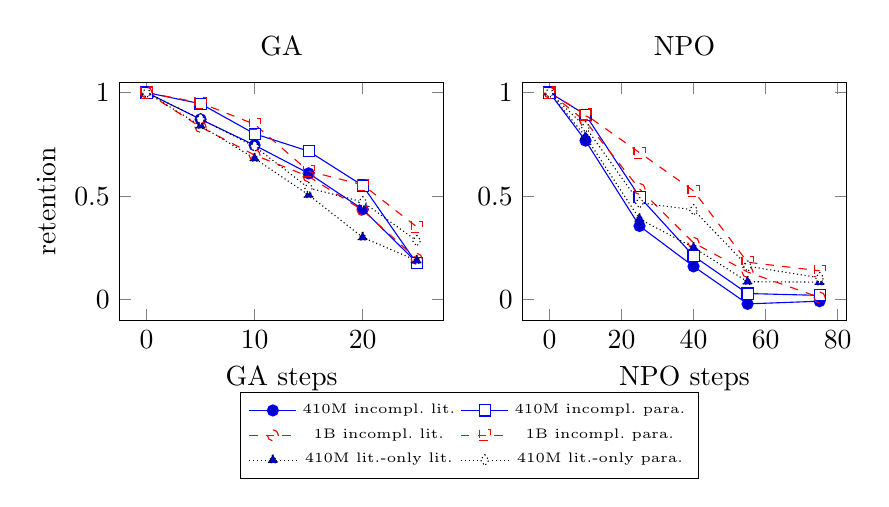
\begin{tikzpicture}
\begin{axis}[name=ga, width=0.47\textwidth, height=0.38\textwidth, xlabel={GA steps},
  ylabel={retention}, ymin=-0.1, ymax=1.05, title={GA}, legend columns=2,
  legend style={font=\tiny, at={(1.08,-0.3)}, anchor=north}]
\addplot+[mark=*, blue] coordinates {(0,1.000) (5,0.871) (10,0.746) (15,0.610) (20,0.437) (25,0.180)};
\addplot+[mark=square*, blue, mark options={fill=white}] coordinates {(0,1.000) (5,0.946) (10,0.801) (15,0.717) (20,0.551) (25,0.176)};
\addplot+[mark=o, red, dashed] coordinates {(0,1.000) (5,0.834) (10,0.698) (15,0.595) (20,0.432) (25,0.197)};
\addplot+[mark=square, red, dashed, mark options={fill=white}] coordinates {(0,1.000) (5,0.950) (10,0.847) (15,0.620) (20,0.555) (25,0.352)};
\addplot+[mark=triangle*, black, densely dotted] coordinates {(0,1.000) (5,0.840) (10,0.682) (15,0.506) (20,0.301) (25,0.189)};
\addplot+[mark=diamond*, black, densely dotted, mark options={fill=white}] coordinates {(0,1.000) (5,0.872) (10,0.740) (15,0.540) (20,0.472) (25,0.285)};
\legend{410M incompl.\ lit., 410M incompl.\ para., 1B incompl.\ lit., 1B incompl.\ para., 410M lit.-only lit., 410M lit.-only para.}
\end{axis}
\begin{axis}[at={(ga.east)}, anchor=west, xshift=1.0cm, width=0.47\textwidth,
  height=0.38\textwidth, xlabel={NPO steps}, ymin=-0.1, ymax=1.05, title={NPO}]
\addplot+[mark=*, blue] coordinates {(0,1.000) (10,0.768) (25,0.356) (40,0.161) (55,-0.020) (75,-0.007)};
\addplot+[mark=square*, blue, mark options={fill=white}] coordinates {(0,1.000) (10,0.893) (25,0.497) (40,0.211) (55,0.030) (75,0.021)};
\addplot+[mark=o, red, dashed] coordinates {(0,1.000) (10,0.861) (25,0.535) (40,0.275) (55,0.134) (75,0.011)};
\addplot+[mark=square, red, dashed, mark options={fill=white}] coordinates {(0,1.000) (10,0.894) (25,0.710) (40,0.526) (55,0.181) (75,0.140)};
\addplot+[mark=triangle*, black, densely dotted] coordinates {(0,1.000) (10,0.788) (25,0.390) (40,0.252) (55,0.087) (75,0.085)};
\addplot+[mark=diamond*, black, densely dotted, mark options={fill=white}] coordinates {(0,1.000) (10,0.834) (25,0.468) (40,0.434) (55,0.162) (75,0.106)};
\end{axis}
\end{tikzpicture}

\caption{Retention of the calibrated literal (filled markers) and paraphrase (open markers)
advantage, normalised by the mean pre-unlearning advantage over eight seeds ($m=384$).}
\label{fig:retention}
\end{figure*}


\paragraph{Retention} The retention of a score is its advantage after unlearning divided by the
mean advantage before unlearning over seeds; per-seed ratios are unstable when a seed's
pre-unlearning paraphrase advantage is close to zero. Table~\ref{tab:retention} reports the
per-seed tests behind Fig.~\ref{fig:retention}. Comparisons that mix a raw literal score with
a calibrated paraphrase score give larger gaps and, for Pythia-1B, a significant one, but the
two scores have different noise and we do not rely on them.

\begin{table}[t]
\centering\footnotesize\setlength{\tabcolsep}{2pt}
\caption{Paraphrase minus literal retention, averaged over the grid of strengths within each
seed; mean $\pm$ standard error over eight seeds, number of seeds with a positive value, and
the Wilcoxon signed-rank $p$ (smallest attainable $0.008$). The first row of each block is the
like-for-like comparison.}
\label{tab:retention}
\resizebox{\columnwidth}{!}{\begin{tabular}{llccc}
\toprule
Experiment & Scores compared & retention gap & seeds $>0$ & $p$ \\
\midrule
410M, incomplete & calibrated vs.\ calibrated & $+0.074\pm0.047$ & 6/8 & 0.195 \\
410M, incomplete & raw vs.\ raw & $+0.077\pm0.033$ & 6/8 & 0.078 \\
410M, incomplete & raw literal vs.\ calibrated paraphrase & $+0.172\pm0.075$ & 6/8 & 0.078 \\
\addlinespace
1B, incomplete & calibrated vs.\ calibrated & $+0.120\pm0.045$ & 6/8 & 0.078 \\
1B, incomplete & raw vs.\ raw & $+0.083\pm0.041$ & 6/8 & 0.109 \\
1B, incomplete & raw literal vs.\ calibrated paraphrase & $+0.163\pm0.051$ & 7/8 & 0.023 \\
\addlinespace
410M, literal only & calibrated vs.\ calibrated & $+0.080\pm0.059$ & 5/8 & 0.250 \\
410M, literal only & raw vs.\ raw & $+0.065\pm0.082$ & 4/8 & 0.641 \\
410M, literal only & raw literal vs.\ calibrated paraphrase & $+0.134\pm0.079$ & 6/8 & 0.195 \\
\bottomrule
\end{tabular}
}
\end{table}

\paragraph{Literal-only design} Table~\ref{tab:clean} gives the audit verdicts for the
literal-only semantic design whose models are used in Table~\ref{M-tab:baselines}. The paraphrase
advantage before unlearning is about half the literal one and falls roughly in step with it;
the literal and the union rule revoke at nearly identical rates, and the union issues on
retraining in $99\%$ of runs.

\begin{table*}[t]
\centering\footnotesize
\caption{Literal-only semantic design, Pythia-410M: mean calibrated advantages $\pm$ standard
errors over eight seeds; fraction of runs revoked by the literal and the union rule and issued
by the union rule ($40$ reveal orders per seed); membership-inference AUC of the organic forget
biographies against the organic holdout (loss score).}
\label{tab:clean}
\resizebox{\textwidth}{!}{\begin{tabular}{lcccccc}
\toprule
Subject & literal $\hat\Delta$ & paraphrase $\hat\Delta$ & rev.\ lit. & rev.\ union & iss.\ union & organic AUC \\
\midrule
none & $+0.292\pm0.017$ & $+0.153\pm0.025$ & 1.00 & 1.00 & 0.00 & 0.55 \\
retrain & $+0.011\pm0.010$ & $+0.031\pm0.020$ & 0.02 & 0.01 & 0.99 & 0.51 \\
\midrule
GA 5 & $+0.245\pm0.016$ & $+0.133\pm0.023$ & 1.00 & 1.00 & 0.00 & 0.53 \\
GA 10 & $+0.199\pm0.018$ & $+0.113\pm0.012$ & 0.96 & 0.96 & 0.04 & 0.51 \\
GA 15 & $+0.148\pm0.020$ & $+0.083\pm0.013$ & 0.68 & 0.67 & 0.33 & 0.49 \\
GA 20 & $+0.088\pm0.026$ & $+0.072\pm0.009$ & 0.25 & 0.25 & 0.75 & 0.50 \\
GA 25 & $+0.055\pm0.029$ & $+0.044\pm0.019$ & 0.13 & 0.10 & 0.90 & 0.49 \\
NPO 10 & $+0.230\pm0.021$ & $+0.128\pm0.018$ & 0.97 & 0.98 & 0.02 & 0.52 \\
NPO 25 & $+0.114\pm0.021$ & $+0.072\pm0.011$ & 0.36 & 0.34 & 0.66 & 0.48 \\
NPO 40 & $+0.074\pm0.013$ & $+0.066\pm0.008$ & 0.06 & 0.04 & 0.96 & 0.48 \\
NPO 55 & $+0.025\pm0.010$ & $+0.025\pm0.018$ & 0.01 & 0.02 & 0.98 & 0.48 \\
NPO 75 & $+0.025\pm0.012$ & $+0.016\pm0.014$ & 0.01 & 0.00 & 1.00 & 0.47 \\
\bottomrule
\end{tabular}
}
\end{table*}

\bibliographystyle{IEEEtranN}
\bibliography{refs}

\end{document}
